\chapter{Background}


\section{Skein Theory}

\subsection{Foundations and General Notions}
In this work, we will be forced to discuss a few different variants of skein modules. For this reason, it will be useful to first describe some general framework of skein theory so that each of these variants will be a special case. Unless otherwise stated, we will assume $M$ is an oriented $3$-manifold with boundary $\partial M$ (possibly empty), $\Sigma$ is an oriented surface, $I$ is the real interval $[0,1]$, $R$ is a commutative and unital ring. 

\begin{definition}
    Let $T_1, T_2: X \to M$ be smooth embeddings of a smooth manifold $X$ into $M$. A \textbf{smooth ambient isotopy} $H: T_1 \Rightarrow T_2$ is a smooth homotopy of diffeomorphisms $H_t: M \to M$ such that $H_0=\id_M$ and $H_1 \circ T_1 = T_2$. Furthermore, we demand that the boundary $\partial M$ is fixed by the homotopy. 
\end{definition}

The relation 
\[
T_1 \sim T_2 \textrm{ if and only if there exists a smooth ambient isotopy } H: T_1 \Rightarrow T_2
\]
is an equivalence relation. The smoothness requirement of $H$ is important when considering knots. Without it, all knots would be equivalent to the unknot by contracting all of the complexity of the knot to a point. 

\begin{definition}
Let $N$ be a finite set of points contained in the boundary $\partial M$. An \textbf{$N$-tangle} in $M$ (or just \textit{tangle} for short) is the smooth ambient isotopy class of a smooth embedding 
\[
T: \underbrace{\underset{j \in J}{\bigsqcup}\, S^1}_{:=L} \sqcup \underbrace{\underset{k \in K}{\bigsqcup}\, I}_{:=B} \to M
\]
for some finite sets $J$ and $K$ such that
\begin{enumerate}
\item the image of $L$ lies in the interior of $M$,
\item the image of the interior of $B$ lies in the interior of $M$,
\item the image of the boundary of $B$ equals $N$.
\end{enumerate}
If $B$ is empty, then the result is called a \textbf{link} in $M$. Similarly, if $L$ is empty, then it's called a \textbf{braid} in $M$. 

One may also consider \textit{oriented} or \textit{framed} tangles by choosing an orientation or framing for each point in $N$ and for each connected component of $L$ and $B$ such that the choices are compatible with each other with respect to the smooth embedding.
%For our purposes, the difference between framed and unframed tangles will be a matter of convention; we choose to work with framed tangles as is standard in the literature. 
If $M = \Sigma \times I$, then we will assume that the points in $N$ are contained in $\Sigma \times \{ \frac{1}{2} \}$ and that their framings are thought to be embedded orthogonally to $\Sigma \times \{ \ast \}$. 
\end{definition}

We say a framed tangle in $\Sigma \times I$ has \textbf{blackboard framing} if the entire framing is embedded orthogonally to $\Sigma$. Every framed link in $\Sigma \times I$ is isotopic to one with a blackboard framing by turning each twist into a loop with a local blackboard framing:

\[
    \vcenter{\hbox{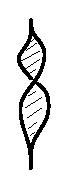
\includegraphics[height=3cm]{twist.eps}}} \quad = \quad \vcenter{\hbox{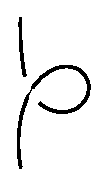
\includegraphics[height=3cm]{invvh2.eps}}}.
\]
This suggests that we may represent framed links in $\Sigma \times I$ as link diagrams on $\Sigma$. Indeed, equivalence under ambient isotopy is captured by the Reidemeister moves 2, 3, and a modified Reidemeister move 1:

\[
    \vcenter{\hbox{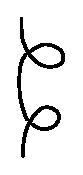
\includegraphics[height=3cm]{modifiedr1.eps}}} \quad = \quad \vcenter{\hbox{
\includegraphics[height=3cm]{modifiedr1resolution.eps}}}.
\]

\AP{Add pictures of RII and RIII for good measure.}
Below are some examples of framed tangle diagrams.

\[
    \vcenter{\hbox{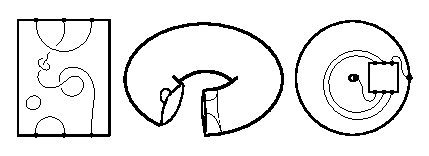
\includegraphics[height=3cm]{Ntangles.eps}}}
\]

Define the \textbf{writhe} of a tangle diagram is the number of positive crossings minus the number of negative crossings. It is easy to see that the Reidemeister moves above preserve the writhe of a diagram, so the concept is well defined. Writhe should be thought of as a grading on the free $R$-module on the set of tangles in the given space, which provides a good reason to work with framed links over ordinary links. Such a module is a main ingredient of this theory, so let's honor it with a proper discussion.

\begin{definition}
Let $\ct(M, N)$ be the free $R$-module generated by the set of framed $N$-tangles in $M$. Analagously, we can define $\ct^{or}(M,N)$ to be the free $R$-module generated by the set of oriented framed $N$-tangles in $M$. All definitions which are to follow in this subsection have an analagous definition using oriented tangles. Also, we will formally define $\cs_R(\varnothing, \varnothing) := R$. 
\end{definition}

The construction $\ct( -, -)$ is actually a symmetric monoidal functor $\ct: \sfc \to R\textsf{-Mod}$ for a careful choice of category $\sfc$ which we now describe. The objects of $\sfc$ are pairs $(M, N)$ of the same type as discussed previously. A morphism $(f, W): (M', N') \to (M, N)$ is a pair of a smooth, orientation-preserving embedding $f: M' \to M$ such that $M - f(M')$ is either a smooth 3-manifold or the empty set, and choice of $W \in \ct\big( M-f(M'), N \sqcup f(N') \big)$ (unless $M - f(M')$ is empty, in which case $W$ is a formal symbol for the "empty link" in the empty set). Composition is given by $(g, W') \circ (f, W) = (g \circ f, W' \cup W)$, which is associative since $\circ$ and $\cup$ are associative.

\AP{Give a picture of composition in $\sfc$.}

The induced map denoted $W: \ct(M', N') \to \ct(M, N)$ is a linear map defined by $W(T) = W \cup T$, and we will refer to such a linear map $W$ as a \textbf{wiring}. We are abusing notation by denoting this linear map by $W$, but it should be clear from the context what $f$ is since it is technically encoded in the data of the element $W \in \ct\big( M-f(M'), N \sqcup f(N') \big)$. It is true that $\ct$ preserves composition and identity morphisms, making and so $\ct$ is functorial. $\sfc$ can now be equipped with a symmetric monoidal structure via disjoint union. It is clear that 
\[\cs_R(M \sqcup M', N \sqcup N') \cong \cs_R(M, N) \underset{R}{\otimes} \cs_R(M', N')\]
for any sets of framed points $N \subset \partial M$ and $N' \subset \partial M'$. The unit is given by the object $(\varnothing, \varnothing) \in \sfc$ and define $\ct(\varnothing, \varnothing) := R$, which makes $\ct$ a symmetric monoidal functor. 

\begin{definition}
Let $B$ be the smooth closed $3$-ball, $N_i$ be a choice of $2i$ boundary points of $B$, and let $X \subset \underset{i \in \N}{\bigsqcup} \ct(B, N_i)$ be some (typically finite) set, which we will call a set of \textbf{skein relations}. Given any tangle module $\ct(M, N_M)$, there exists a submodule $\ci(X)$ generated by the set 
\[\{ W(x) \mid x \in X \text{ and } W:\ct(B, N_B) \to \ct(M, N_M) \text{ is a wiring diagram} \}.\] 
A quotient of the form $\cs_X(M, N) := \ct(M, N) / \ci(X)$ is called a \textbf{skein module} of $M$ relative to $N$. If $N = \varnothing$ is the empty set, we may use the notation $\cs_X(M) := \cs_X(M, \varnothing)$. Similar definitions may be given using oriented and/or unframed tangles instead. 
\end{definition}
The construction $\cs_X(-, -)$ is a functor in the same way that $\ct(-, -)$ is; a smooth, orientation-preserving embedding $f: M \to M'$ and an element $W \in \cs_X\big( M-f(M'), N \sqcup f(N') \big)$ defines a linear map $W: \cs_X(M, N) \to \cs_X(M', N')$. In fact, the quotient maps $\alpha_{(M, N)}: \ct(M, N) \to \cs_X(M, N)$ yield a natural transformation. In other words, given a morphism $(M, N) \to (M', N')$ in $\sfc$, the diagram
\begin{center}
\begin{tikzcd}
	\ct(M, N) \arrow[d,"\alpha_{(M, N)}"] \arrow[r, "W"] 
	& \ct(M', N') \arrow[d, "\alpha_{(M', N')}"]\\
	\cs_X(M, N) \arrow[r, "W"] & \cs_X(M', N')
\end{tikzcd}
\end{center}
commutes. Such a functor will be called a $\textbf{skein theory}$ (or \textit{oriented} skein theory if the skein relations are based on oriented tangles). 

For any oriented surface $\Sigma$, we can define a category $\sfskein_X(\Sigma)$ which we will call a $\textbf{skein category}$. The objects of this category are finite sets of framed points (together with a choice of orientation if the skein theory is oriented) $N$ in $\Sigma$, and the morphisms $N \to N'$ are elements of $\cs_X\big(\Sigma \times I, (N \times \{0\}) \sqcup (N' \times \{1\})\big)$, so the category is $R$-linear. Write composition of morphisms by concatenation. If $y:N \to N'$ and $z:N' \to N''$ are morphisms, then their composite $yz:N \to N''$ is constucted by gluing $z$ on $y$ through $N'$ and rescaling the interval coordinate appropriately.

\AP{Picture of composition in $\sfskein_X(\Sigma)$.}

The endomorphism algebras in this category are called \textbf{skein algebras} and are denoted by $\cs_X(\Sigma, N) := \cs_X(\Sigma \times I, (N \times \{0\}) \sqcup (N \times \{1\}) \big)$. If $N$ is the empty set, then we reduce the notation to simply $\cs_X(\Sigma)$.

If $f: \Sigma \to \Sigma'$ is a smooth embedding of surfaces, then there is an induced functor 
\[
\sfskein_X(f): \sfskein_X(\Sigma') \to \sfskein_X(\Sigma)
\]
defined on objects by $\sfskein_X(f)(N) = f(N)$ and on morphisms in the following way. First, extend $f$ trivially to $f \times \id_I: \Sigma \times I \to \Sigma' \times I$. Then, in the skein algebra of the complement of the image of $f \times \id_I$, choose the multiplicative identity element $e \in \cs_X\big( \Sigma' - \im(f) \big)$ which is the empty tangle. The pair $(f \times \id_I, e)$ is an object in the category $\sfc$, which gives rise to a wiring
\[e: \cs_X\Big(\Sigma \times I, \big(N \times \{0\}\big) \sqcup \big(N' \times \{1\}\big) \Big) \to \cs_X\Big(\Sigma' \times I, \big(f(N) \times \{0\}\big) \sqcup \big( f(N') \times \{1\} \big) \Big)\]
via the functor $\cs_X$. Now we may define what $\sfskein_X(f)$ does to morphisms: $\sfskein_X(f)(y) = e(y)$ for any $y \in \cs_X\Big(\Sigma \times I, (N \times \{0\}) \sqcup (N' \times \{1\}) \Big)$.

\AP{Picture of how $\sfskein_X(f)$ works on morphisms.}

It is clear that $\sfskein_X(f)$ preserves composition and identity morphisms. Therefore, if we let $\mathsf{Surf}$ be the category of smooth embeddings between smooth oriented surfaces, we can summarize our last few points by saying we have a functor
\[
\sfskein_X: \mathsf{Surf} \to \mathsf{Cat}.
\]
In particular, $\sfskein_X(f)$ defines algebra homomorphisms on the skein algebras
\[e: \cs_X\big(\Sigma, N\big) \to \cs_X\big(\Sigma', f(N)\big).\]
\AP{We use this type of algebra homomorphism when we embed the annulus into the torus.}

The above homomorphisms are a special case of a more general type of map. If $N$ is a set of framed points on $\Sigma$, then a smooth embedding $f: \Sigma \to \partial M$ induces a $\cs_X(\Sigma, N)$-module structure on $\cs_X\big(M, N'\big)$ for any $N'$ with $f(N) \subseteq N'$. The action is given by ``pushing tangles in through the boundary". In other words, the pre-composition of a smooth embedding of a collar neighborhood $g: \partial M \times I \to M$ with $f \times \id_I: \Sigma\times I \to \partial M \times I$ induces a bilinear map
\[
\cs_X(\Sigma, N) \times \cs_X(M, N') \to \cs_X(M, N')
\]
because $M$ minus a collar neighborhood is diffeomorphic to itself. Alternatively, a choice of element in $\cs_X(\Sigma, N')$ produces a wiring $\cs_X(M, N') \to \cs_X(M, N')$.

\AP{Picture of action.}

\subsection{Examples of Skein Theories}

The last subsection leaves us with an important and unanswered question. Which sets of skein relations $X$ produce interesting skein theories? One class of examples is found by examing sets of relations satisfied by morphisms in a linear ribbon category. Ribbon categories are braided monoidal categories which are rigid and equipped with a twist morphism for every object, satisfying some compatibility conditions. The axioms are such that the morphisms may be interpreted as framed braid diagrams. In particular, the morphisms satisfy the Reidemeister moves shown previously. We will discuss three examples of skein theories derived from skein relations which are meant to emulate linear relations satisfied by the braid and twist morphisms in certain ribbon categories coming from the representation theory of quantum groups, a topic which has generated a lot of interest from mathematicians since the 1980s. Quantum groups provided a class of non-commutative and non-cocommutative Hopf algebras which are not constructed in a trivial way (such as taking a tensor product of one non-commutative and one non-cocommutative Hopf algebra). Furthermore, the categories of representations of quantum groups are braided monoidal categories with non-involutive braidings. The skein relations below capture how far off the braidings are from being involutive.  

Here, we are forced to fix a base ring. For our purposes, $R$ must be a commutative ring containing invertible elements $s$ and $v$. Typical choices of $R$ are $\Z[s^{\pm 1}, v^{\pm 1}], \Q(s, v)$, or some other ring in between these.  In particular, the theorem \AP{Cite BB} is stated over this ring, a result we will depend heavily on later on. \\

\begin{example}[\textit{Kauffman (Dubrovnik) Skein Relations}]
Let $X'$ denote the set of two unoriented skein relations
\begin{flalign*}
    (1) \quad \vcenter{\hbox{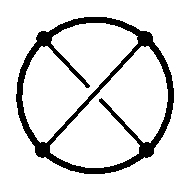
\includegraphics{poscross.eps}}} &= \vcenter{\hbox{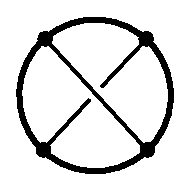
\includegraphics{negcross.eps}}} + (s-s^{-1}) \,\, \vcenter{\hbox{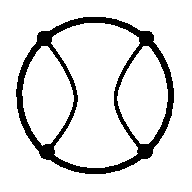
\includegraphics{idresolution.eps}}} - (s-s^{-1}) \,\, \vcenter{\hbox{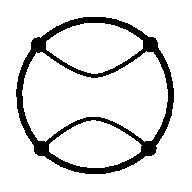
\includegraphics{capcupresolution.eps}}} \\ \\
    (2) \quad \vcenter{\hbox{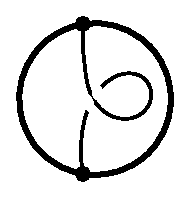
\includegraphics{vh.eps}}} &= v \,\, \vcenter{\hbox{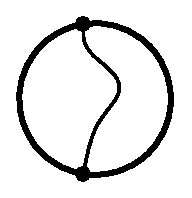
\includegraphics{frameresolution.eps}}}.
\end{flalign*}
The functor $\cd(-,-) := \cs_{X'}(-,-)$ is the Dubrovnik skein theory (sometimes just called the Kauffman skein theory). We will use the notation $\mathsf{D} := \sfskein_{X'}$ for the Dubrovnik skein categories. Using the Dubrovnik variant is important for us (see \AP{universal enveloping algebra result}). This theory is related to Dubrovnik polynomials in that the Dubrovnik polynomial of a link is a normalized value of the link in $\cd(S^3)$. The normalization is often so that the Dubrovnik polynomial of the unknot is $1$, whereas the value of the unknot in $\cd(S^3)$ is $\delta_\cd := 1 - \frac{v-v^{-1}}{s-s^{-1}}$, which can be deduced from the skein relations.
\end{example}

\begin{example}[\textit{HOMFLYPT Skein Relations}]
Next, let $X''$ denote the set of two oriented skein relations
\begin{flalign*}
    (1) \quad \vcenter{\hbox{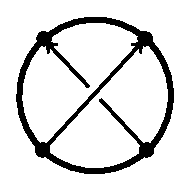
\includegraphics{poscrossor.eps}}} &= \vcenter{\hbox{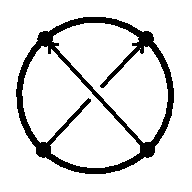
\includegraphics{negcrossor.eps}}} + (s-s^{-1}) \,\, \vcenter{\hbox{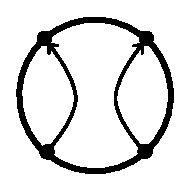
\includegraphics{idresolutionor.eps}}} \\ \\
    (2) \quad \vcenter{\hbox{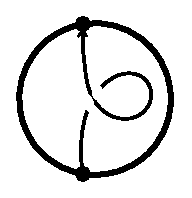
\includegraphics{vhor.eps}}} &= v \,\, \vcenter{\hbox{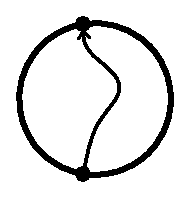
\includegraphics{frameresolutionor.eps}}}.
\end{flalign*}
The functor $\ch(-,-) := \cs_{X''}(-,-)$ is the HOMFLYPT skein theory and we use the notation $\mathsf{H} := \sfskein_{X''}$ for the HOMFLYPT skein categories. As in the Dubrovnik case, this theory is related to HOMFLYPT polynomials so that the HOMFLYPT polynomial of a link is a normalized value of the link in $\ch(S^3)$. Again, some often make the choice to normalize this polynomial so that the value of the unknot is $1$, but the value of the unknot in $\ch(S^3)$ is $\delta_\ch := -\frac{v-v^{-1}}{s-s^{-1}}$.
\end{example}

\begin{example}[\textit{Kauffman Bracket Skein Relations}]
As a final example, let $X'''$ denote the set of two unoriented skein relations
\begin{flalign*}
    (1) \quad \vcenter{\hbox{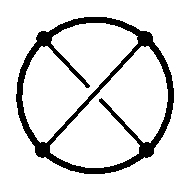
\includegraphics{poscross.eps}}} &= s \,\, \vcenter{\hbox{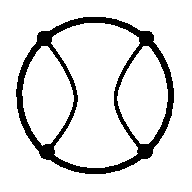
\includegraphics{idresolution.eps}}} + s^{-1} \,\, \vcenter{\hbox{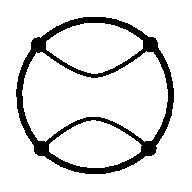
\includegraphics{capcupresolution.eps}}} \\ \\
    (2) \quad \vcenter{\hbox{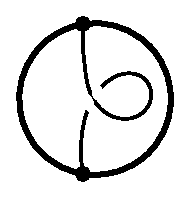
\includegraphics{vh.eps}}} &= -s^{-3} \,\, \vcenter{\hbox{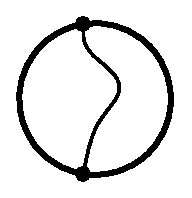
\includegraphics{frameresolution.eps}}}.
\end{flalign*}
The functor $\ck(-,-) := \cs_{X'''}(-,-)$ is the Kauffman bracket skein theory (not be confused with the Kauffman skein theory) and we use $\mathsf{K} := \sfskein_{X'''}$ to notate the Kauffman bracket skein categories. The value of a link in $\ck(S^3)$ is equal to its bracket polynomial, which may be normalized as above to obtain its Jones polynomial. 
\end{example}

\begin{remark}
Any linear combination of tangles which satisfy the Dubrovnik skein relations will also satisfy the Kauffman bracket skein relations after making the specialization $v=-s^{-3}$. Therefore, there is a natural transformation of skein theories $\eta: \cd(-,-) \to \ck(-,-)$ induced by the intentity map on link diagrams. 
\end{remark}

In this work, we will be focused on generalizing existing results from the HOMFLYPT and Kauffman bracket skein theories to the Dubrovnik skein theory, but we will state a few facts regarding the HOMFLYPT and Kauffman bracket skein theories when it is valuable for us to do so. 

\subsection{Skein algebras of tangles in a cube}

In the case where $\Sigma = I \times I$, the endomorphism objects of $\mathsf{D}(\Sigma), \mathsf{H}(\Sigma)$, and $\mathsf{K}(\Sigma)$ are known and provide the motivation for why the choices of skein relations are what they are. For an integer $n \geq 1$, let $[n]$ be a set of $n$ points in $\Sigma$, chosen to be evenly spaced along the line segment $\frac{1}{2} \times I$ (choose all points share the same orientation in the context of an oriented skein theory). Then the endomorphism algebras 
\[
BMW_n := \End_\mathsf{D}(\Sigma)([n]), \qquad H_n := \End_\mathsf{H}(\Sigma)([n]), \qquad TL_n := \End_\mathsf{K}(\Sigma)([n])
\]
are known to be isomorphic to the Birman-Murakami-Wenzl, (Type A) Hecke, and Temperley-Lieb algebras, respectively (\AP{*Add citations}). 

Let $q \in \C$ be not a root of unity, $U_q(\mathfrak{gl}_N)$ be the Drinfeld-Jimbo quantum group associated to the Lie algebra $\mathfrak{gl}_N$, and $V$ be the natural representation of $U_q(\mathfrak{gl}_N)$ (\AP{cite CP}). Then $H_n$ acts on the $n$-fold tensor product $V^{\otimes n}$ by $U_q(\mathfrak{gl}_N)$-linear endomorphisms, and this action generates $\End_{U_q(\mathfrak{gl}_N)}(V^{\otimes n})$. This is actually part of the statement of quantum Frobenius-Schur-Weyl duality: $V^{\otimes n}$ is a $U_q(\mathfrak{gl}_N)$-$H_n$-bimodule, and the action of one algebra generates the linear endomorphisms with respect to the other. So a representation of one algebra determines a representation of the other via tensor product with $V^{\otimes n}$. The Birman-Murakami-Wenzl algebra plays the role of the Hecke algebra for $U_q(\mathfrak{g}_N)$ in the case where $\mathfrak{g}$ is one of the orthogonal or symplectic Lie algebras. For this reason, from a Lie theoretic point of view, the HOMFLYPT skein theory is thought of as a ``type A" theory, while the Dubrovnik skein theory is a ``types B, C, D" skein theory.

As for the Temperley-Lieb algebra $TL_n$, it acts on the $n$-fold tensor power $V^{\otimes n}$ of the natural representation of $U_q(\mathfrak{gl}_2)$. Actually, there is a surjective algebra homomorphism $\pi_{TL}: H_n \to TL_n$ and the action $H_n \to \End_{U_q(\mathfrak{gl}_2)}(V^{\otimes n})$ factors through this homomorphism (see \AP{cite Jimbo}). One can conclude that the action of $H_n$ on $V^{\otimes n}$ is not faithful, at least in the case when $N=2$ and $n \geq 1$. \AP{sl2 vs gl2?}

Much is known about these algebras and some of the results surrounding them are very useful in our context. One of the main ideas is that each of the algebras discussed above has a family of idempotents which provide algebraically nice closures to links in the skein algebra of an annulus. Let's first describe the Hecke algebra in more detail before focusing on the BMW algebra. 

For any partition $\lambda$ of $n$, there exists an element $y_\lambda \in H_n$ which is idempotent, so that $y_\lambda^2 = y_\lambda$, and minimal in the sense that it generates a minimal left-ideal of $H_n$ (see \AP{cite Aiston-Morton}). The elements $h_n := y_{(n)}$ corresponding to single row partitions are called \textbf{(Hecke) symmetrizers}. These elements have a certain absorption property which makes them unique, which we will now describe. Let us use $\sigma_i \in H_n$ be the positive crossing between the $i^{\rm{th}}$ and $(i+1)^{\rm{th}}$ strands. 
\AP{Picture of oriented $\sigma_i \in H_n$.}
The algebra $H_n$ is generated by the $\sigma_i$ and the symmetrizers are the unique idempotent elements satisfying $\sigma_i h_n = s h_n = h_n \sigma_i$. In this way, $h_n$ corresponds to a $1$-dimensional representation of $H_n$ (it is a deformation of the trivial representation of $\C S_n$ where $s=1$).

A similar story holds for the BMW algebra. Firstly, $BMW_n$ is generated by positive crossing elements $\sigma_i$ and cap-cup elements $c_i$. 
\AP{pictures of $\sigma_i$ and $c_i$}
The $c_i$ generate a proper ideal $I_n$ in $BMW_n$. In (\AP{cite BB}), the authors show that the complement of $I_n$ in $BMW_n$ is isomorphic to $H_n$, giving an isomorphism $BMW_n \cong H_n \oplus I_n$. Then they construct an additive and multiplicative (but non-unital) homomorphism 
\[
\Gamma_n : H_n \to BMW_n
\]
which is a section of the natural projection $BMW_n \to H_n$ such that 
\begin{equation} \label{eq:bbsectionproperty}
\Gamma_n(x)y = 0 = y \Gamma_n(x) \quad \textrm{for } x \in H_n, y \in I_n.
\end{equation}
Using this section, one can transport the minimal idempotents $y_\lambda \in H_n$ to minimal idempotents $\tilde{y}_\lambda := \Gamma_n(y_\lambda) \in BMW_n$. The elements $\tilde{h}_n := \tilde{y}_{(n)}$ are called the \textbf{(BMW) symmetrizers} and are the unique idempotent elements of $BMW_n$ satisfying the properties of the Hecke symmetrizers and property \eqref{eq:bbsectionproperty}. 

\AP{Come back and add braiding/twist identities from BB if we need them.}


\AP{This diagram actually doesn't commute... $\pi_H(c_i)=0, but \eta_{\dots}(c_i) = c_i.}
\begin{center}
\begin{tikzcd}
	& BMW_n \arrow[dl, "{\pi_H}", two heads] \arrow[dd, "{\eta_(I^3, 2n)}", two heads] \\
H_n \arrow[dr, "{\pi_{TL}}", two heads] \arrow[ur, "\Gamma", bend left, hook] & \\
	& TL_n
\end{tikzcd}
\end{center}

\subsection{Skein algebras of the annulus}



\subsection{HOMFLYPT and Kauffman Skein Modules}

\subsection{Skein Algebras of the Annulus}

\subsection{A Relative Skein Algebra of the Annulus}

\subsection{The HOMFLYPT Skein Algebra of the Torus}



\section{The Ring of Symmetric Functions}

\subsection{Character Rings of Classical Groups}

\subsection{Bases of $\Lambda$ and Identities}